
%%%%%%%%%%%%%%%%%%%%%%%%%%%%%%%%%%%%%%%%%%%%%%%%%%%%%%%%%% 
%%%   Find a Nice Title: #Seen #Storytelling #Events   %%%
%%%%%%%%%%%%%%%%%%%%%%%%%%%%%%%%%%%%%%%%%%%%%%%%%%%%%%%%%%

\documentclass{sig-alternate}

\usepackage{url}
\usepackage{textcomp}
\usepackage{listings}
\usepackage{color}
\usepackage{multirow}

% listing styles
\lstset{numbers=left, numberstyle=\tiny,basicstyle=\ttfamily\scriptsize, tabsize=2, keywordstyle=\underbar, stringstyle=\small, backgroundcolor=\color[gray]{0.94}, framexleftmargin=2pt}
\lstdefinestyle{rdfa}{numberblanklines=true, morekeywords={}}

% Turtle box
\definecolor{olivegreen}{rgb}{0.2,0.8,0.5}
\definecolor{grey}{rgb}{0.5,0.5,0.5}
\lstdefinelanguage{ttl}{
sensitive=true,
morecomment=[l][\color{grey}]{@},
morecomment=[l][\color{olivegreen}]{\#},
morestring=[b][\color{blue}]\",
keywordstyle=\color{cyan},
morekeywords={version,owl,rdf,rdfs,xml,xsd,dbpedia,dbo,str,sso,scms,fr,ld}
}
\lstset{
        basicstyle=\ttfamily\scriptsize,
        upquote=true,
        showspaces=false,
        showstringspaces=false,
        showtabs=false,
        tabsize=2,
        frame=none,
        breaklines,
        numbers=none,
        framexleftmargin=2mm,
        xleftmargin=2mm,
}

\newcommand{\hilight}[1]{\colorbox{yellow}{#1}}
\newcommand{\todo}[1]{\colorbox{red}{#1}}

%%%%%%%%%%%%%%%%%%%%%%%%%%%%%%%
%%%  Beginning of document  %%%
%%%%%%%%%%%%%%%%%%%%%%%%%%%%%%%

\begin{document}

\title{Storifying Events with Timelines of Links}

\numberofauthors{3}
\author{
\alignauthor Carlo Andrea Conte\\
	\affaddr{Mahaya Inc.}\\
    \affaddr{New York, USA}\\
    \email{carloante@msn.com}
\alignauthor Mor Naaman\\
    \affaddr{Cornell Tech}\\
    \affaddr{New York, USA}\\
    \email{mor.naaman@cornell.edu}
\alignauthor Rapha\"el Troncy\\
	\affaddr{EURECOM}\\
	\affaddr{Biot, France}\\
	\email{raphael.troncy@eurecom.fr}	\\
}

\maketitle

%%%%%%%%%%%%%%%%%%
%%%  Abstract  %%%
%%%%%%%%%%%%%%%%%%

\begin{abstract}
% Motivation: story is being told with links which are being shared. Describe the links processing algorithms, architecture, engineering. Describe the two algorithms that extract links (based on volume, based on velocity).

Social media platforms constitute a valuable source of information regarding real-world happenings. In particular, user generated contents on mobile-oriented platforms like Twitter allow for real-time narrations thanks to the instantaneous nature of their publishing. A common trend is to publish links to more exhaustive articles, media files and other types of information sources. In this paper, we will describe a system able to listen for tweets published regarding a particular event, for which a time-range and a set of specific hashtags are known. Such system will extract, resolve and eventually filter all the links according to a velocity-based function and a volume-based function. For each selected link, relevant information will be scraped from the referenced page.

\todo{Write conclusions reached}

\end{abstract}

% A category with the (minimum) three required fields
\category{H.3.1}{Information Storage and Retrieval}{Content Analysis and Indexing}
%\terms{Algorithms,Measurement,Experimentation,Web}
\keywords{Event, Story, Content Analysis, Seen, Twitter, Hashtags, Links}

%%%%%%%%%%%%%%%%%%%%%%%%%
%%%  1. Introduction  %%%
%%%%%%%%%%%%%%%%%%%%%%%%%

\section{Introduction}
\label{sec:introduction}

\todo{Mention real-time and low-latency requirements}

\todo{we mention we only use tweets and why (see comment)}
% The reason why only tweets are taken into account is that Twitter includes in every tweet's data a list of entities. Such list contains a number of meaningful items parsed from the original text. Typical examples include hashtags and, luckily for us, web urls. Another reason for this choice is that users are more likely to publish links via Twitter than via Instagram, as the latter is a service strongly centered on content creation.

\todo{Mention we don't cover the logic for gathering tweets (see comment)}
%...as we build our experiment on top of Seen's constantly updated database. \cite Wired's article about Seen

\todo{Also mention we don't cover logic for general event metadata, we use Seen's db}

% -How people talk on Twitter about events
% -Problem of noise, quantity, quality
% -Problem of real-time computation
% -Introducing paper's sections

Twitter, Facebook, Instagram, and other social platforms provide a continuous stream of user-contributed messages and media. Very often, contents are not generated within the platform itself, but are referenced via hyperlinks. The nature of these pages can be various: they can include images, news articles, real-time video streams and many other types of content. It is possible to obtain elements related to a particular event when specific keywords and time ranges are known. Filtering the results according to their relevance, and aggregating them in a storyline, can lead to a rich narration of the event thanks to the use of a very diverse set of media.

In this document we will describe a system that aims at extracting a timeline of links from a stream of tweets. These links will be filtered in order to reduce the noise and surface valuable information. In addition to this, they will be complemented by metadata scraped from their referenced pages: this metadata can then be used to represent the timeline in an intelligible way.

After introducing similar and related projects in Section \ref{sec:related-work}, we will discuss the general architecture of the system we implemented in Section \ref{sec:architecture}. This section will also describe the implementation of the two score processors we used for our tests. Section \ref{sec:experiment} will comment the results of our experiments. Finally, in Section \ref{sec:storyline} we will see a few examples of storylines based on the results obtained in Section \ref{sec:experiment}.

%%%%%%%%%%%%%%%%%%%%%%%%%
%%%  2. Related Work  %%%
%%%%%%%%%%%%%%%%%%%%%%%%%

\section{Related Work}
\label{sec:related-work}

\todo{Raphael, Mor}

%%%%%%%%%%%%%%%%%%%%%%%%%
%%%  3. Architecture  %%%
%%%%%%%%%%%%%%%%%%%%%%%%%

\section{Architecture}
\label{sec:architecture}
% This section can be shortened, I'll decide when the first draft of the paper is ready and I can see how long it is

The system we propose has to be able to run in real time in order to make it possible to build storylines of events that are happening in the moment of the analysis. Because of this we also want results to be returned with the smallest delay possible since the moment raw data first entered the system. These requirements impose the adoption of an efficient, flexible concurrency model, that would be easily scalable according to the data flow. At the same time, it must be possible to process past events with the same algorithm, as results should be consistent regardless the moment the event takes place.

As we already mentioned in Section \ref{sec:introduction}, we won't cover the interface this system has with the original source of data. We will assume that a separated process keeps updating our database at regular intervals with raw data from Twitter. In our testing environment, Twitter is queried for contents for a given event about every 15 minutes, although this frequency can significantly fluctuate depending on the number of events being tracked by the system at the same time. We used a MongoDB database, where raw data was indexed according to creation time and mentioned hashtags.

The different steps implemented by the process we are describing comprehend:
\begin{enumerate}
 \item Extracting links from a collection of tweets according to the parameters identifying an event, namely a set of hashtags and a timerange,
 \item Resolving these links to their canonical form,
 \item Ranking links and apply a first basic filter,
 \item Collecting useful data from the pages referenced by the links selected,
 \item Outputting a timeline of links featuring real-time filtering functions.
\end{enumerate}
We will now detail the general architecture of this system. Figures \ref{fig:architecture_resolution} and \ref{fig:architecture_metadata} are a graphical representation of the blocks building up the software.
\begin{figure}[htbp]
  \centering
  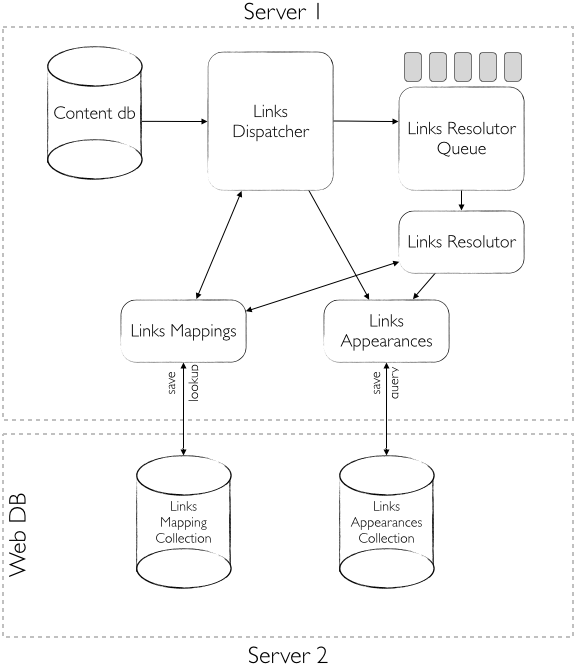
\includegraphics[width=6cm]{Figures/links_processing_architecture_resolution.png}
  \caption{Architecture - From extraction to resolution.}
  \label{fig:architecture_resolution}
\end{figure}
\begin{figure}[htbp]
  \centering
  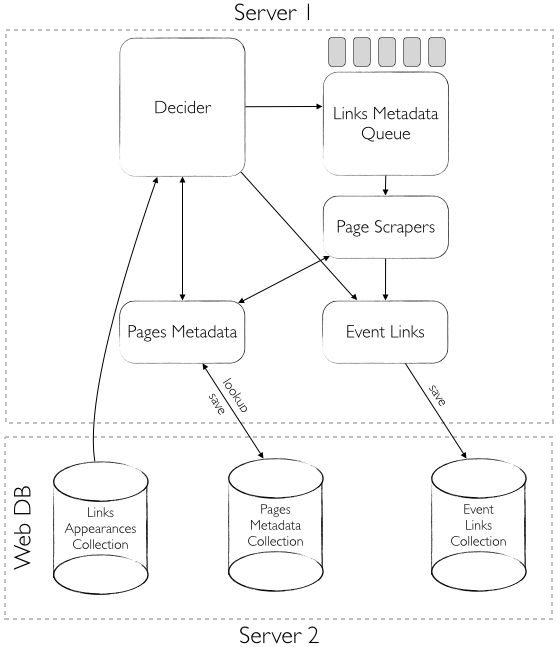
\includegraphics[width=6cm]{Figures/links_processing_architecture_metadata.png}
  \caption{Architecture - From ranking to page scraping.}
  \label{fig:architecture_metadata}
\end{figure}

The complete process for each link implies two very severe bottlenecks: the url resolution and the page scraping. In order to overcome this limitation and build a more efficient system, we split the logic in different parts intended to run in parallel.

The \emph{links dispatcher} (Figure \ref{fig:architecture_resolution}) represents the first step of this processing chain. It retrieves from the \emph{content database} all the tweets for a particular temporal window and containing any of the hashtags included in a given set. After loading the raw data, the links dispatcher extracts every link from the tweets' entities (\cite{RestTweetsDoc}), it queries the \emph{links mappings} class to check if such URL has been resolved already. If it hasn't, it places it in a \emph{links resolutor queue}, otherwise it adds it together with information about its tweet to the \emph{links appearances}. The links dispatcher can be run on happening events, by computing the temporal window's length according to the time of the previous processing, but it can also process past events, by using a sliding window algorithm where the window has a pre-defined size that adjusts itself to handle slow processing cases.

The links resolutor queue is a Redis queue\cite{RedisQueues} of jobs. This means that a list of pointers to python functions and their arguments is stored in a Redis database for later execution. The processes responsible of reading job queues and executing them are called ``workers''. The advantages of this approach resides in the fact that many workers instances can be run at the same time, and their number and behavior can be adjusted according to the workload. This allows for great flexibility in the way the system can be scaled depending on the abundancy of data.

All the urls in the links resolutor queue will be resolved by the \emph{links resolutor} function. This function will first look the url up in the links mappings and, if it is not found, it resolves the url and eventually saves a new mapping. This resolution step is necessary because most links on Twitter are shortened by various url shortener services (sometimes provided by Twitter itself). When a link is successfully resolved, it is added to the \emph{links appearances} and a new mapping is saved.

The \emph{links appearances} class manages an unnormalized collection of all the resolved links. Every item contains information about the url, the tweet that contained it and the event that url was for. In fact, multiple items might carry data about the same combination of url and tweet as long as they reference different events.

Links appearances are periodically accessed by the \emph{decider} (Figure \ref{fig:architecture_metadata}), which is responsible of ranking them and filtering them as needed. The computation is always done on a sliding temporal window of fixed size, and only for links of one event at a time. The scoring system relies on \emph{links score processors} for its decision process: different score processors can be implemented for testing different score functions. We will detail the links score processors used for our experiments in Sections \ref{sec:volume_based_links_selection} and \ref{sec:velocity_based_links_selection}. The LSPs\footnote{Links Score Processors} we will use only implement a very basic first filtering: their main function in the experiments discussed in this paper will consist in enriching the event links with features useful for ranking. More consisten filtering possibilities will be provided by our front-end interface.

If a link is selected for publication, the decider queries the \emph{pages metadata} class for any available metadata for that link. If no metadata is available, the link appearance is added to the \emph{Links Metadata Queue}, otherwise it is saved together with its metadata as an \emph{event link}. The decider can either be run in real time on happening events, or it can simulate the same sliding window algorithm on past events.

The \emph{Links Metadata Queue} is processed by the \emph{metadata scraper}. This function extracts the domain from the url and selects a scraper class accordingly, it loads the referenced page and extracts pieces of information from it (e.g. a title, a description and a representative image). Different scrapers look for different tags in the DOM structure, as different websites usually expose different information in different ways. In our tests, we will use a generic scraper that collects information stored in Open Graph and Twitter Cards meta-tags. Only links for which enough metadata is found are saved as event links while the pages metadata collection is updated accordingly. Event link duplicates are avoided, while their scores and other relevant features are updated to the latest result.

The final results of this system are stored in the event links collection. This dataset holds all the links together with their score and other attributes infered by the link score processor used to rank them (e.g. total volume, highest volume in a time-window duration etc...). In addition to this, the same record contains the metadata extracted from the referenced page and the id of the event for which that link was processed. In fact, the same link can appear multiple times as long as it referenced different events.

\subsection{Front-end Interface}
The results of this processing will all be displayed on a simple javascript interface, under the form of a storyline: the list of links will be sorted chronologically according to a \emph{display time} field defined by the LSP. A filtering functionality will make it possible to select a cutoff score for the links to be visualized. This interface also draws a pie-chart representing the source domains of the links displayed (taking into account the filtering parameter).

Figure \ref{fig:javascript_interface.png} shows a very simple example of the storyline.\todo{Screenshot} The attributes shown for every link must be interpreted according to the LSP that produced them, this will be explained after introducing each LSP. It is more clear thanks to this example one reason why our system scrapes information from every page: any visual representation will take advantage of it to make the list more human readable. Moreover, the combination of an image and a description can offer a more complete information than a tweet alone.

One additional feature implemented by this interface is the aggregation of information regarding the source domain of every item: this attribute is added by the metadata scraping process to every link, and it is included in the HTML structure of the page via data attributes to be read and charted by the javascript application. We will make use of these charts when discussing our tests' results.

\subsection{Volume based LSP}
\label{sec:volume_based_links_selection}
\todo{Using again the volume threshold based on the number of items instead?}
Organizing a collection of every single appearance of every link gives us the possibility to obtain information about the volume of shares reached by a link during the event. As an example, Figure \ref{fig:batkid_whitehouse_volume} shows the number of appearances in time of the link to president Obama's Vine for Batkid\footnote{An initiative of Make-A-Wish Foundation for a child affected by leukemia and that attracted the attention of social media: http://abcnews.go.com/US/batkids-make-transforming-san-francisco-gotham/story?id=20899254}.
\begin{figure}[htbp]
  \centering
  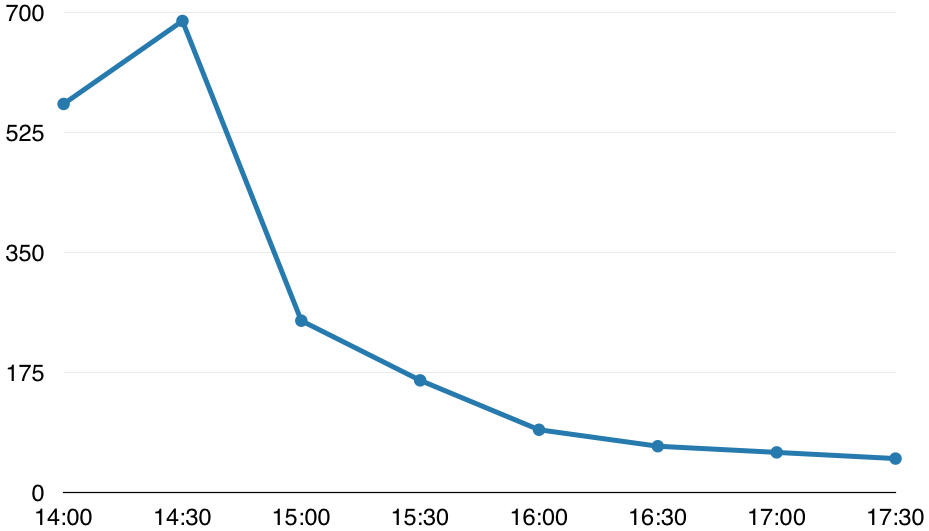
\includegraphics[width=\linewidth]{Figures/batkid_whitehouse_volume.png}
  \caption{Volume of president Obama's Vine video for Batkid shares.}
  \label{fig:batkid_whitehouse_volume}
\end{figure} \todo{Higher time-resolution excel graph}

The volume based LSP assigns to every link a score equal to the cumulative function of its volume throughout the event. A very basic filtering step is implemented by a manually chosen volume threshold that is only meant to exclude the noise of links that did not trigger any interest at all in the audience, and can be considered to be background noise (e.g. those links with only one appearance). A link that has been shared at a nearly constant rate during the analyzed time range will be more likely to appear in our timeline than a link that reached a very high volume at a particular point in time. The display time for links ranked by this LSP is choosen to be the time of the earliest appearance that passed the elementary filtering (e.g. the second appearance of a link).

\subsection{Velocity based LSP}
\label{sec:velocity_based_links_selection}
The velocity based LSP computes links' scores as the appearances volume reached by a link within one decider processing time window. The decider's time windows occur every 20 minutes and are 30 minutes long, thus allowing a 10 minutes overlap between each window. \todo{After experimenting a bit, decide between using the ranking for filtering or the volume.}

This LSP implements the same filter described in Section \ref{sec:volume_based_links_selection}, with the only difference that the threshold is compared with the current time window's volume. The display time is defined as the first time a link appearance survives the filtering for the first time in a time window. However, the score is always updated to the highest volume the link has reached within a window.

%%%%%%%%%%%%%%%%%%%%%%%%
%%%  4. Experiments  %%%
%%%%%%%%%%%%%%%%%%%%%%%%

\section{Experiments}
\label{sec:experiment}
In this section we describe the experiments made to evaluate the efficacy of the storylines built using our method, and to compare the results obtained with different LSPs (Sections \ref{sec:volumeResults} and \ref{sec:velocityResults}). In Section \ref{sec:dataset} we clarify what system constitutes the data source for our experiments, as well as how data is structured in such system.

\subsection{Dataset}
\label{sec:dataset}
The data used in our experiments is provided by Seen\footnote{http://seen.co}, a service that aims at organizing social media by building automatic summaries of events \cite{SeenWired}.
%Describe what the dataset is (Seen's dataset), how data is not already organized by event, but the events database gives us the necessary info to split it.

\subsection{Volume based LSP experimental results}
\label{sec:volumeResults}

Volume graphs of some approved links, explanations, interpretation of the reasons

\subsection{Velocity based LSP experimental results}
\label{sec:velocityResults}

Cross validation: In the previous two subsections we can pretty much only validate the precision of the two algorithms together. How about considering the set of elements that were not selected in one algorithm, but were selected in the other one and vice versa to see if one has a better recall?

%%%%%%%%%%%%%%%%%%%%%%%%%%%%%%%%%
%%%  5. Building a Storyline  %%%
%%%%%%%%%%%%%%%%%%%%%%%%%%%%%%%%%

\section{Building a Storyline}
\label{sec:storyline}
We should place the selected links (selected based on any method we decided was better for this scope between the previous two) in chronological order and see if they actually follow the evolution of the story, with what granularity. This will only work with a long event.


%%%%%%%%%%%%%%%%%%%%%%%%%%%%%%%%%%%%%%%
%%%  6. Conclusion and Future Work  %%%
%%%%%%%%%%%%%%%%%%%%%%%%%%%%%%%%%%%%%%%

\section{Conclusion and Future Work}
\label{sec:conclusions}


\section{Acknowledgments}
\label{sec:ack}

\nocite{*}
\bibliographystyle{abbrv}
\bibliography{seen}
\balancecolumns
% That's all folks!
\end{document} 
